\documentclass[./main]{subfiles}

\begin{document}
  \chapter{Private key encryption.}

  This encryption scheme achieves information-theoric security.

  \begin{defn}[Symmetric encryption]
    Let $\mathcal{K}$ be a key space, $\mathcal{P}$ be a plain-text space and let $\mathcal{C}$ be a ciphertext space
    These three spaces are finite spaces.

    A \textit{symmetric encryption} scheme over $(\mathcal{K}, \mathcal{P}, \mathcal{C})$ is a tuple of three algorithms $(\mathrm{KeyGen}, \mathrm{Enc}, \mathrm{Dec})$ :
    \begin{itemize}
      \item $\mathrm{KeyGen}$ provides a sample $k$ of $\mathcal{K}$;
      \item $\mathrm{Enc} : \mathcal{K} \times \mathcal{P} \to \mathcal{C}$;
      \item $\mathrm{Dec} : \mathcal{K} \times \mathcal{C} \to \mathcal{P}$.
    \end{itemize}
    Without loss of generality, we will assume that $\operatorname{im} \mathrm{Enc} = \mathcal{C}$.
    We want to ensure \textbf{Correctness}: for any key $k \in \mathcal{K}$ and message $m \in \mathcal{P}$, we have that:
  \[
    \mathrm{Dec}(k, \mathrm{Enc}(k, m)) = m
    .\]

    The elements $m$ and $k$ are independent random variables and all the elements in $\mathcal{K}$ and $\mathcal{P}$ have non-zero probability.
  \end{defn}

  \begin{rmk}
    The algorithm $\mathrm{Enc}$ could (and should\footnote{If the algorithm is deterministic, if we see two identical ciphers we know that the messages are identical, and this can be seen as a vulnerability of this protocol.}) be probabilistic.
    However, the algorithm $\mathrm{Dec}$ is deterministic.
    
    So far, we did not talk about efficiency of these algorithms.
  \end{rmk}

  \begin{defn}[Shannon, 1949]
    A symmetric encryption scheme is said to have \textit{perfect security} whenever, for any $\bar{m}$ and any $\bar{c}$, 
    \[
      \Pr_{k,m}[m = \bar{m}  \mid \mathrm{Enc}_k(m) = \bar{c}] = \Pr_{m}[m = \bar{m}]
    .\] 
  \end{defn}

  The intuition is that knowing the encrypted message tells me \textit{nothing} about the message.

  \begin{lem}[Shannon]
    Given a symmetric encryption scheme $(\mathrm{KeyGen}, \mathrm{Enc}, \mathrm{Dec})$ has perfect security then $|\mathcal{K}| \ge |\mathcal{P}|$.
  \end{lem}
  \begin{prv}
    Let $\bar{c} \in \mathcal{C}$ and define \[
    \mathcal{S} := \{\bar{m} \in \mathcal{P}  \mid \exists \bar{k} \in \mathcal{K}, \bar{m} = \mathrm{Dec}(\bar{k}, \bar{c})\}
    .\]
    Let $N := |\mathcal{S}|$.
    We have that $N \le |\mathcal{K}|$ as $\mathrm{Dec}$ is deterministic.
    We also have that $N \le |\mathcal{P}|$ as $\mathcal{S} \subseteq \mathcal{P}$.
    Finally, assume $N < |\mathcal{P}|$.
    This means, there exists $\bar{m} \in \mathcal{P}$ such that $\bar{m} \not\in \mathcal{S}$.
    Then, 
    \[
      \Pr[m = \bar{m}  \mid \mathrm{Enc}_k(m) = \bar{c}] = 0
    ,\] 
    but by assumption, $\Pr[m = \bar{m}] \neq 0$.
    So this is not a perfectly secure scheme.
    We can conclude that \[
    N = |\mathcal{P}| \le |\mathcal{K}|
    .\] 
  \end{prv}

  \begin{exm}[One-Time PAD]
    Let $\mathcal{K} = \mathcal{C} = \mathcal{P} = \{0, 1\}^{\ell}$.
    Here are the algorithms used:
    \begin{itemize}
      \item $\mathrm{KeyGen}$ samples from $\mathcal{U}(\{0,1\}^\ell)$.
      \item $\mathrm{Enc}(k, m)$ we compute the XOR $c = m \oplus k$.
      \item  $\mathrm{Dec}(k,m)$ we compute the XOR $m = c \oplus k$.
    \end{itemize}
  \end{exm}

  \begin{thm}
    The One-Time PAD is a perfectly-secure symmetric encryption.
  \end{thm}
  \begin{prv}
    \begin{description}
      \item[Correctness.]
        We have that
        \[
        \mathrm{Dec}(k, \mathrm{Enc}(k, m)) = k \oplus k \oplus m = m
        .\]
      \item[Security.]
        We have, by independence of $m$ and $k$ we have that
        \begin{align*}
          \Pr[m = \bar{m}  \mid \mathrm{Enc}(k, m) = \bar{c}]
          &= \Pr[m = \bar{m}  \mid k \oplus m = \bar{c} ]\\
          &= \Pr[m = \bar{m}]
        .\end{align*}
    \end{description}
  \end{prv}

  \begin{rmk}
    This example is not practical:
    \begin{itemize}
      \item keys need to be larger than the message;
      \item you cannot encrypt twice: for example, $c_1 = m_1 \oplus k$ and $c_2 = m_2 \oplus k$, then we have $c_1 \oplus c_2 = m_1 \oplus m_2$.
    \end{itemize}
    This last part is why that protocol is called a \textit{One-Time secure encryption}.
  \end{rmk}

  We want to be able to encrypt arbitrarily long messages!
  We will have to make a trade-off and we choose to not care about \textit{perfect} security.
  Why? In real life, we don't care about proving that something is proven to be absolutely infeasible, we only want to believe it is infeasible in practice.
  \begin{center}
  \textbf{\textit{Computational complexity} is sufficient in practice.}
  \end{center}
  Let us be more precise in the next section.

  \section{Pseudo-random generators.}

  \begin{defn}
    Let $\mathcal{D}_0$ and $\mathcal{D}_1$ be two distributions over $\{0,1\}^n$.

    An algorithm $\mathcal{A} : \{0,1\}^n \to \{0,1\}$ is called a \textit{distinguisher} between $\mathcal{D}_0$ and $\mathcal{D}_1$. We define its \textit{distinguishing advantage} as:
    \[
      \mathrm{Adv}_\mathcal{A} := \big| \underbrace{\Pr_{x \gets \mathcal{D}_1} [\mathcal{A}(X) = 1]}_{ \mathclap{\substack{\text{probability of}\\ \text{being right}}} } - \underbrace{\Pr_{x \gets \mathcal{D}_0} [\mathcal{A}(X) = 1]}_{\mathclap{\substack{\text{probability of}\\ \text{being mistaken}}}} \big|
    .\] 

    We say that $\mathcal{D}_0$ and $\mathcal{D}_1$ are \textit{computationally indistinguishable} if for any efficient distinguisher $\mathcal{A}$ its advantage $\mathrm{Adv}_\mathcal{A}$ is small.
    We will write, in this case, $\mathcal{D}_1 \simeq^\mathrm{c} \mathcal{D}_2$.
  \end{defn}

  This definition is not very formal yet, we have not defined "efficient" and "small."
  This can be formalized by introducing a parameter $\lambda \in \mathds{N}$ called the \textit{security parameter}.

  \begin{defn}
    Let $(\mathcal{D}_{0, \lambda})_{\lambda \in \mathds{N}}$ and $(\mathcal{D}_{1, \lambda})_{\lambda \in \mathds{N}}$ be two distributions over $\{0,1\}^{n(\lambda)}$ for a non-decreasing polynomial $n(\lambda)$.
    The value of $\lambda \in \mathds{N}$ is called the \textit{security parameter}.

    An algorithm $\mathcal{A} : \{0,1\}^{n(\lambda)} \to \{0,1\}$ is called a \textit{distinguisher} between the distributions $\mathcal{D}_{0, \lambda}$ and $\mathcal{D}_{1, \lambda}$. We define its \textit{distinguishing advantage} as:
    \[
      \mathrm{Adv}_\mathcal{A}(\lambda) := \big| \underbrace{\Pr_{x \gets \mathcal{D}_{1, \lambda}} [\mathcal{A}(X) = 1]}_{ \mathclap{\substack{\text{probability of}\\ \text{being right}}} } - \underbrace{\Pr_{x \gets \mathcal{D}_{0, \lambda}} [\mathcal{A}(X) = 1]}_{\mathclap{\substack{\text{probability of}\\ \text{being mistaken}}}} \big|
    .\] 

    We say that $\mathcal{D}_{0, \lambda}$ and $\mathcal{D}_{1, \lambda}$ are \textit{computationally indistinguishable} if for any distinguisher $\mathcal{A}$ running in $\mathrm{O}(\lambda^c)$ for some $c > 0$\footnote{This means it is polynomial in $\lambda$, which we will write $\mathrm{poly}(\lambda)$} its advantage $\mathrm{Adv}_\mathcal{A}$ is a $\mathrm{o}(1 / \lambda^c)$ for some $c > 0$.\footnote{This means it is negligible in terms of $\lambda$, which we will write $\mathrm{negl}(\lambda)$.}
  \end{defn}
  
  Our goal now is to extend the One-Time PAD to messages $m$ larger than the key $k$.
  We want to construct some function $G$ that takes as input the key $k \in \{0,1\}^n$ and expend it to a string $G(k) \in \{0,1\}^\ell$  for some $\ell > k$ that is computationally hard to distinguish from a uniform random string.
  This is called a \textit{PGR} or \textit{pseudo-random generator}.

  \begin{defn}
    A \textit{pseudo-random generator} is a pair of poly-time algorithms $(\mathrm{Setup}, G)$ such that:
    \begin{itemize}
      \item $\mathrm{Setup}$ is an algorithm that takes as input a security parameter $\lambda$ (taken as a string $1^\lambda$ of length $\lambda$, \textit{i.e.}\ we write $\lambda$ in unary) and returns a public parameter;
      \item $G_\lambda : \{0,1\}^{n(\lambda)} \to \{0,1\}^{\ell(\lambda)}$ is an algorithm which takes a string $k$ of length $n(\lambda)$ and return a string $G(k)$ of length $\ell(\lambda)$ with $\ell(\lambda) > n(\lambda)$.
    \end{itemize}
    such that
    \begin{itemize}
      \item $G$ is deterministic;
      \item $\ell(\lambda) > n(\lambda)$ (we say that it is \textit{expanding})
      \item the distributions $\{\mathcal{U}(\{0,1\}^{\ell(\lambda)})\}_{\lambda \in \mathds{N}}$ and $\{G(\mathcal{U}(\{0,1\} ^{n(\lambda)}))\}_{\lambda \in \mathds{N}}$ are computationally indistinguishable (we call it \textit{pseudo-randomness}).
    \end{itemize}
  \end{defn}

  Another way of defining a pseudo-random generator is with \textit{unpredictability} instead of \textit{pseudo-randomness}.
  \begin{defn}
    This is the same definition as before but replacing pseudo-randomness with \textit{unpredictability}.

    A PRG $(\mathrm{Setup}, G)$ is \textit{unpredictable} if, for any index $i \in \{0, \ldots, \ell(\lambda)\}$ and any efficient adversary $\mathcal{A} : \{0,1\}^{n} \to \{0,1\}$, we have that:
    \[
    \Big|
    \Pr_{k \gets \mathcal{U}(\{0, 1\}^{n(\lambda)} } \big[\mathcal{A}(G(k)_{|i}) = G(k)_{i+1}\big] - \frac{1}{2}
    \Big| = \mathrm{negl}(\lambda)
    .\]
  \end{defn}

  We can now prove that the two definitions are equivalent.

  \begin{thm}
    The two definitions of a PRG are equivalent.
  \end{thm}
  \begin{prv}
    To simplify, we will remove the security parameter from the notations.

    On one side, assume we have a predictor $\mathcal{A} : \{0,1\}^i \to \{0,1\}$ that succeeds in guessing $G(k)_{i+1}$ with non-negligible probability.
    We then construct a distinguisher $\mathcal{B}$ against pseudo-randomness as $\mathcal{B}$ receive a sample $x$ from either $\mathcal{D}_0 = \mathcal{U}(\{0,1\}^\ell)$ or $\mathcal{D}_1 = G(\mathcal{U}(\{0,1\}^n))$:
    algorithm $\mathcal{B}$ runs $\mathcal{A}$ on input  $x_{|i}$ and checks if $\mathcal{A}(x_{|i}) \overset ? = x_{i+1}$.
    In that case, $\mathcal{B}$ will return $1$; otherwise it returns $0$.
    What is the advantage of $\mathcal{B}$?
    \begin{align*}
      \mathrm{Adv}_{\mathcal{B}} &=
      \big| \Pr_{x \gets \mathcal{D}_1}[\mathcal{B}(x) = 1] - \overbrace{\Pr_{x \gets \mathcal{D}_0}[\mathcal{B}(x) = 1]}^{1 / 2} \big| \\
      &= \big| \Pr_{x \gets \mathcal{D}_1}[\mathcal{A}(x_{|i}) = x_{i+1}] - \frac{1}{2} \big|
    .\end{align*}
    This is the definition of the predictability advantage of $\mathcal{A}$ (which is non-negligible by assumption).

    Next, we will use a technique called an \textit{Hybrid Argument} (due to Yao in '82).
    Assume we have a distinguisher $\mathcal{A}$ such that \[
      \mathrm{Adv}_\mathcal{A} = \big| \Pr_{x \gets \mathcal{D}_1}[\mathcal{A}(x) = 1] - \Pr_{x \gets \mathcal{D}_0}[A(x) = 1]\big|
    \]
    is non-negligible, say $\mathrm{Adv}_\mathcal{A} \ge \varepsilon$.
    We then define $\ell + 1$ distributions $(\mathcal{D}_i)_{i = 0, \ldots, \ell}$ as
    \[
    \mathcal{D}_i := \mleft\{\,x \in \{0,1\}^\ell \;\middle|\;
      \begin{array}{l}
        x_{|i} = G(k)_{|i} \text{ for } k \gets \mathcal{U}(\{0,1\}^n)\\
        x_{|i+1, \ldots, \ell} \gets \mathcal{U}(\{0,1\}^{\ell - i})
      \end{array}
    \,\mright\} 
    .\]
    We then have, by all the terms cancelling (this is a telescoping sum), that:
    \begin{align*}
      \varepsilon \le \mathrm{Adv}_\mathcal{A}(\mathcal{D}_0, \mathcal{D}_n)
      &= \Big|\sum_{i = 0}^\ell \big(\Pr_{x \gets \mathcal{D}_{i+1}}[\mathcal{A}(x) = 1] - \Pr_{x \gets \mathcal{D}_i}[\mathcal{A}(x) = 1]\big)\Big| \\
      &\le \sum_{i = 0}^\ell \big|\Pr_{x \gets \mathcal{D}_{i+1}}[\mathcal{A}(x) = 1] - \Pr_{x \gets \mathcal{D}_i}[\mathcal{A}(x) = 1]\big|\\
      &\le \sum_{i= 0}^\ell \mathrm{Adv}_\mathcal{A}(\mathcal{D}_i, \mathcal{D}_{i+1})
    .\end{align*}
    By the pigeonhole principle, we have that there exists an $i \in \{0,\ldots,\ell\}$, such that \[
      \big|\Pr_{x \gets \mathcal{D}_{i+1}}[\mathcal{A}(x) = 1] - \Pr_{x \gets \mathcal{D}_i}[\mathcal{A}(x) = 1] \big| \ge \frac{\varepsilon}{\ell + 1}
    .\] 
    As $\varepsilon$ is non-negligible and  $\ell + 1$ being polynomial in $\lambda$, we have that $\varepsilon / (\ell + 1)$ is non-negligible.
    How to turn this into a predictor for $i$?
    Let us define $\mathcal{B}_i$ as a predictor which is given $G(k)_{|i}$ and supposed to predict $G(k)_{i+1}$.
    Algorithm $\mathcal{B}_i$ will computes $x \in \{0,1\}^\ell$ with $x \gets G(k)_{|i} \mathop{||} y $ where $y \gets \mathcal{U}(\{0,1\}^{\ell-i})$.
    Then $\mathcal{B}_i$ runs algorithms $\mathcal{A}$ on input $x$, and $\mathcal{A}$ returns a bit  $b \in \{0,1\}$ and $\mathcal{B}_i$ outputs a prediction $x_{i+1}$ for $G(k)_{i+1}$ if $b = 1$ and  $1 - x_{i+1}$ otherwise.
    What is the prediction advantage of $\mathcal{B}_i$?
    \begin{align*}
      &\phantom{={}}\Pr[\mathcal{B}_i(G(k)_{|i}) = G(k)_{i+1}]\\
      &= \Pr \left[
        \begin{array}{c}
          \mathcal{A}(x) = 0 \land x_{i+1} = 1 - G(k)_{i+1}\\
          \lor\\
          \mathcal{A}(x) = 1 \land x_{i+1} = G(k)_{i+1}
        \end{array}
      \right] \\
      &= \Pr_{x \gets \mathcal{D}_i} [\mathcal{A}(x) = 0 \land x_{i+1} = 1 - G(k)_{i+1}]\\
      &\quad + \Pr_{x\gets \mathcal{D}_i}[\mathcal{A}(x) = 1 \land x_{i+1} = G(k)_{i+1}]\\
      &=
      \frac{1}{2} \Pr_{x \gets \bar{\mathcal{D}}_{i+1}}[\mathcal{A}(x) = 0]
      + \frac{1}{2} \Pr_{x \gets \mathcal{D}_{i}}[\mathcal{A}(x) = 1]\\
      &= \frac{1}{2}\big(
        \Pr_{x \gets \mathcal{D}_{i+1}}[\mathcal{A}(x) = 1]
        + 1 - \Pr_{x \gets \bar{\mathcal{D}}_{i+1}}[\mathcal{A}(x) = 1]
      \big) \\
    .\end{align*}
    where we write $\bar{\mathcal{D}}_{i+1}$ is the "flipped" of $\mathcal{D}_{i+1}$.
    We have that:
    \begin{align*}
      &\phantom{={}}\Pr_{x \gets \mathcal{D}_i}[\mathcal{A}(x) = 1]\\
      &= \Pr_{x \gets \mathcal{D}_i}[\mathcal{A}(x) = 1 \land x_{i+1} = G(k)_{i+1}] \\
      &\quad+ \Pr_{x \gets \mathcal{D}_i}[\mathcal{A}(x) = 1 \land x_{i+1} = 1 - G(k)_{i+1}] \\
      &= \frac{1}{2}\big(\Pr_{x \gets \mathcal{D}_i}[\mathcal{A}(x) = 1] + \Pr_{x \gets \bar{\mathcal{D}}_{i+1}}[\mathcal{A}(x) = 1]\big)
    ,\end{align*}
    thus
    \[
      \Pr_{x \gets \bar{\mathcal{D}}_{i+1}}[\mathcal{A}(x) = 1] = 2 \Pr_{x \gets \mathcal{D}_i}[\mathcal{A}(x) = 1] - \Pr_{x \gets \mathcal{D}_{i+1}}[\mathcal{A}(x) = 1]
    .\]
    Hence, 
    \begin{align*}
      \Pr[\mathcal{B}_i(G(k)_{|i}) - G(k)_{i+1}] =& \\
      \frac{1}{2}\Pr_{x \gets \mathcal{D}_{i+1}}[\mathcal{A}(x) = 1] +{} &1 - 2 \Pr_{x \gets \mathcal{D}_i}[\mathcal{A}(x) = 1] + \Pr_{x \gets \mathcal{D}_{i+1}}[\mathcal{A}(x) = 1]
    .\end{align*}
    Finally, we can conclude that:
    \[
      \mathrm{Adv}_\mathcal{A}(\mathcal{D}_i, \mathcal{D}_{i+1}) = \Big|\Pr[\mathcal{B}_i(G(k)_{|i}) = G(k)_{i+1}] - \frac{1}{2}\Big| \ge \frac{\varepsilon}{n}
    .\] 
  \end{prv}

  \begin{exm}
    Let us go back to the One-Time PAD example.
    As said before, to get information-theoretic security, one needs the key's bit length to be no smaller than the message's length.
    
    Now, how do we use the PRG to have a secure protocol?
    We encode using the PRG:
    \[
    \mathrm{Enc}_k(m \in \{0,1\}^\ell) = m \oplus G(k) \in \{0,1\}^\ell
    .\]
    We can use a key of length $128$ bits but encode a $1\:\mathrm{Gb}$ message.

    If we have a PRG $G : \{0,1\}^n \to \{0,1\}^{n+1}$ where $n$ is the length of the key, then we can call $G$ on itself a lot of times to get a string of any length~$\ell > n$. (This is likely to be proven in the tutorials.)\footnote{The teacher gave us an explanation on how we can double the length of a string, then it is easy to go from $128$ to $2^{30}$ bits. However, that construction is still using the $n \to n + 1$ construction  $2^{23}$ times.}
  \end{exm}

  As seen before with the One-Time PAD, this kind of encryption can only be used once: you cannot re-use the key to encrypt multiple messages.


  \begin{defn}
    An encryption scheme $(\mathrm{KeyGen}, \mathrm{Enc}, \mathrm{Dec})$ is called \textit{secure against a single message chosen plain-text attack} if, for all polynomial-time adversary $\mathcal{A}$, and all $m_0, m_1$ chosen by $\mathcal{A}$, we have that the two distributions are computationally indistinguishable:
    \[
      \big( \mathrm{Enc}(k, m_0) \big)_{k \gets \mathrm{KeyGen}(\,)} \simeq^\mathrm{c} \big( \mathrm{Enc}(k, m_1) \big)_{k \gets \mathrm{KeyGen}(\,)}
    .\]
  \end{defn}

  \begin{rmk}
    Another way of thinking about this kind of security is to imagine two players, the adversary $\mathcal{A}$ and the challenger $\mathcal{C}$.
    \begin{itemize}
      \item The challenger generates a secret key $k \in \{0,1\}^n$ (which we assume to be uniform) and a uniform bit $b \gets \mathcal{U}(\{0,1\})$.
      \item The adversary give two messages $m_1$ and $m_2$ to $\mathcal{C}$.
      \item Then, the challenger encrypt $m_b$ using the key, and gives it to  $\mathcal{A}$.
      \item Finally, $\mathcal{A}$ tries to "guess" $b$ (\textit{i.e.}\ which message was encrypted ($m_0$ or $m_1$).
    \end{itemize}
    Writing $b^\star$ for the guess of the adversary, we obtain a different formulation for the advantage of $\mathcal{A}$ :
    \[
    \mathrm{Adv}(\mathcal{A}) = \big| 2 \times \Pr[b^\star = b] - 1 \big|
    .\]
    This definition of the advantage is equivalent (\textit{c.f.}\ tutorials) to the one used before :
    \[
      \mathrm{Adv}(\mathcal{A}) = \big|{\Pr[\mathcal{A} \text{ guesses } 1  \mid b = 0]} - \Pr[\mathcal{A} \text{ guesses } 1  \mid b = 1]\big|
    .\] 
  \end{rmk}

  \begin{prop}
    The PRG-based construction is secure against a single message chosen plain-text attack.
  \end{prop}
  \begin{prv}
    We want to show that, if there is an attacker against the PRG-based scheme, then there is a distinguisher fo the PRG.
    We will use the "encryption security game" analogy in this proof.
    We define two games:
    \begin{itemize}
      \item Let $\mathrm{Hybrid}_0$ be the game where $\mathcal{C}$ uses $m_0$.
      \item Let $\mathrm{Hybrid}_4$ be the game where $\mathcal{C}$ uses $m_1$.
    \end{itemize}
    which we then complete with three other "intermediate" games:
    \begin{itemize}
      \item Let $\mathrm{Hybrid}_1$ be the game similar to $\mathrm{Hybrid}_0$ except that $c = m_0 \oplus G(k)$ is replaced by $c = m_0 \oplus u$ where $u \gets \mathcal{U}(\{0,1\}^\ell)$.
      \item Let $\mathrm{Hybrid}_2$ be the game similar to $\mathrm{Hybrid}_1$ except that $m_0$ is changed with $m_1$ and thus $c = m_1 \oplus u$.
      \item Let $\mathrm{Hybrid}_3$ be the game similar to $\mathrm{Hybrid}_2$ except that $c = m_1 \oplus u$ is replaced with $c = m_1 \oplus G(k)$.
    \end{itemize}
    We define \[
      p_n := \Pr[\mathcal{A} \text{ guesses $1$ in the game } \mathrm{Hybrid}_n]
    .\] 
    The goal is to show that $|p_0 - p_4|$ is negligible.
    To prove that we will prove that $|p_0 - p_1|$, $|p_1 - p_2|$, $|p_2 - p_3|$ and $|p_3 - p_4|$ are all negligible (we will then conclude by the triangle inequality).
    This strategy is called \textit{Game Hopping}.
    By symmetry, we only need to consider $|p_0 - p_1|$ and $|p_1 - p_2|$.

    \begin{itemize}
      \item Consider the games $\mathrm{Hybrid}_0$ and $\mathrm{Hybrid}_1$.
        If $\mathcal{A}$ can see the difference between the two cyphers, then it can be used to break the PRG.
        To prove this, we proceed by reduction.
        We introduce a new player, $\mathcal{B}$, who will pretend to be $\mathcal{A}$ from the point of view of $\mathcal{C}$ and \textit{vice-versa}.

        The players are then:
        \begin{itemize}
          \item $\mathcal{A}$ is the encryption adversary;
          \item $\mathcal{C}$ is the PRG challenger;
          \item $\mathcal{B}$ is both the encryption challenger and the PRG adversary.
        \end{itemize}
        We consider two cases: the "PRG" case and the "Uniform" case (depending on the choice for the key used to cypher the message.
        From the point of view of $\mathcal{A}$,
        \begin{itemize}
          \item in the "PRG" case, it should be exactly as in $\mathrm{Hybrid}_0$;
          \item in the "Uniform" case, it should be exactly as in $\mathrm{Hybrid}_1$.
        \end{itemize}
        The game will take place in the following way:
        \begin{itemize}
          \item $\mathcal{A}$ will give $\mathcal{B}$ two messages $m_0$ and $m_1$;
          \item $\mathcal{C}$ will give $\mathcal{B}$ a key $y$ with the required length (either generated uniformly in the "Uniform" case, or with the PRG in the "PRG" case).
          \item $\mathcal{B}$ encrypts the message $m_0$ using the key $y$, and gives it to $\mathcal{A}$.
          \item $\mathcal{A}$ sends its guess $b^\star$ to $\mathcal{B}$, who directly sends it to $\mathcal{C}$.
        \end{itemize}
        Because $\mathcal{A}$'s view is consistent, it behaves as unexpected in $\mathrm{Hybrid}_0$ or $\mathrm{Hybrid}_1$.
        This means that: 
        \begin{itemize}
          \item in the "PRG" case, $\mathcal{B}$ outputs $1$ iff $\mathcal{A}$ outputs $1$, which happens with probability $p_0$.
          \item in the "PRG" case, $\mathcal{B}$ outputs $1$ iff $\mathcal{A}$ outputs $1$, which happens with probability $p_1$.
        \end{itemize}
        If $|p_0 - p_1| = |\Pr[\mathcal{B} \gets 1  \mid \text{PRG case}] - \Pr[\mathcal{B} \gets 1  \mid \text{Uniform case}]|$ is non-negligible, then $\mathcal{B}$ breaks the PRG.
        And, if $\mathcal{A}$ is efficient, so is $\mathcal{B}$.
        Thus, if the PRG is secure, then $|p_0 - p_1|$ is negligible.
      \item For the games $\mathrm{Hybrid}_1$ and $\mathrm{Hybrid}_2$, we will prove that $p_1 = p_2$.
        As $u$ is chosen uniformly, then $\mathcal{A}$ receives a uniform cypher $c$ in both games.
        Then, as $\mathcal{A}$ has the same view, it has the same behavior.
        The rest of the proof is exactly the one for the perfect security of the One-Time PAD.
    \end{itemize}
  \end{prv}

  \section{How to get PRGs? Cryptographic assumptions.}

  One example of a PRG is called RC4 (defined by Rivest in '87).
  It has some weaknesses.
  This PRG was used in WEP, an very old WiFi protocol (still used by 2 \% of WiFi routers), and it has been totally broken (the WEP protocol added weaknesses  on top of RC4's).
  It is also used by Bittorent.
  The state of the art is Salsa20 (software) or Trivium (hardware).

  \begin{defn}
    A function $f : \{0,1\}^k \to \{0,1\}^\ell$ is called \textit{one way} (with no relation between $l$ and $k$ ) if it is computable in polyomial-time and 
    for any polynomial-time adversary $\mathcal{A}$, its advantage \[
      \mathrm{Adv}(\mathcal{A}) = \Pr_{x \gets \mathcal{U}(\{0,1\}^k)}[\mathcal{A}(f(x)) = x' \text{ where } f(x) = f(x') ]
    \]
    is negligible.
  \end{defn}

  We have that:
  \begin{itemize}
    \item if there exists a PRG, then there is a one-way function
    \item if there is a one-way function, then there is a PRG (Goldreich-Levin hard-cord bits).
  \end{itemize}
  There also exists explicit universal functions: if a one-way function exists, then the universal function is one way.

  This problem is connected to the $\mathbf{P}$ \textit{vs.}\ \textbf{NP} problem (existence of one-way function implies $\mathbf{P} \neq \mathbf{NP}$).

  \begin{defn}[Discrete Logarithm Problem, DLP]
    The DLP is defined relative to a prime-order cyclic group $G$ with a generator~$g \in G$.
    This means that \[
    G = \{g^k  \mid k = 0, \ldots, p - 1\} 
    ,\] 
    where $p = |G|$ is a prime number. The group $G$ and the element $g$ are publicly known.
    The goal is, given $h \in G$, find a $x$ such that $g^x = h$.
  \end{defn}

  \begin{exm}
    In $(\mathds{Z} / p \mathds{Z}, +)$, the DLP problem is quite easy.

    In $G_p := ((\mathds{Z} / p \mathds{Z})^\times, \times)$ is cyclic of order $p-1$, but $p-1$ is not necessarily a prime!
    We take a prime $p$ such that $p = 2q + 1$ where $q$ is prime (such primes are called \textit{safe primes}).
    We have that 
    \[
      G_p = \{g, g^2, g^3, \ldots, g^{p-1}\}
    \] and \[G_q = \{(g^2)^0, (g^2)^2, \ldots, (g^2)^k, \ldots, \overbrace{(g^2)^{(p-1) / 2}}^{p^q}\} 
    .\] 
    The group $G_q$ is cyclic with prime order $q$. To find a generator for $G_q$, we simply sample uniformly an element $g_0$ of $(\mathds{Z} / p \mathds{Z})^\star$, then take $h := g_0^2$.
    This is in fact a generator as long as $g_0 \not\in \{-1, 1\}$.
  \end{exm}

  In the 2000s, cryptographers started using the group of elements of an elliptic curve over a finite field.
  For prime order subgroups of $((\mathds{Z} / p \mathds{Z})^\star, \times )$, the best known algorithms cost 
  \[
    \exp(\tilde{\mathrm{O}}(\sqrt[3]{\ln |G|} )) \ll \exp(\mathrm{O}(\ln |G|))
  .\]
  The other cost is for generic "black box" groups (hardness of DLP).
  This blackbox algorithm is the best known algorithm for elliptic curves with $\log_2 |G| \approx 256$.

  Thus, $p$ and $q$ have to be quite large to be hard-to-solve (around $4\,096$ bits) on the case of prime order subgroups of $(\mathds{Z} / p \mathds{Z})^\star$.
  Given $h = g^x$, there is a baby-step-giant-step algorithm to find $x$.
  \begin{itemize}
    \item We start by computing $\{g^0, g, g^1, \ldots, g^{\sqrt{q}}\} $ (baby steps);
    \item Then, we compute $\{h g^{-\sqrt{q}},  hg^{-2\sqrt{q}}, hg^{-3\sqrt{q}}, \ldots, hg^{-\sqrt{q} \sqrt{q} }\} $ (giant steps).
  \end{itemize}
  The cost for each step is around $\sqrt{q}$.
  As $h = g^x = g^{x_0 + \sqrt{q} x_1}$, then we have that $g^{x_0} = h \cdot g^{\sqrt{-q} x_1}$.
  Each of these elements is in one set.

  Then, if we find two elements $g^{x_0}$ in the baby steps and $h \cdot g^{-\sqrt{q} x_1}$ in the giant steps that are equal, then we get $h = g^{x_0} \cdot g^{\sqrt{q} x_1} = g^{x_0 + \sqrt{q} x_1}$, thus we solve the DLP solution.

  That's a $\mathrm{O}\big(\sqrt{|G|}\big)$ time algorithm for finding the DLP.\footnote{The intersection of two lists of length $\sqrt{|G|}$ can be easily done in $\mathrm{O}\big(\sqrt{|G|}\big)$ by using a hashmap, for example, to check if there are collisions.}\showfootnote

  \begin{defn}[Computational Diffie-Hellman Problem, CDH]
    The CDH problem is defined as taking as input $g$ a generator of a group $G$, and two elements $g^a$ and  $g^b$.
    The goal is to find $g^{ab}$.
    This is not as easy as computing $g^a \cdot g^b$ as it'd give us $g^{a+b}$ which is generally different from $g^{ab}$.
  \end{defn}

  If DLP can be easily solved, then so is CDH: we say CDH \textit{reduces} to DLP.
  The other direction is still an open problem, with partial results by Mauer and Wolf in '99.

  \begin{defn}[Decisional Diffie Hellman, DDH]
    The DDH is the problem defined by the following.
    It takes as input three elements $h_1$, $h_2$ and $h_3$ of $G$ either uniformly chosen (\textit{i.e.}\ $g^a, g^b, g^c$ for  $a,b,c \gets \mathcal{U}(\mathds{Z} / p \mathds{Z})$) or of the form $(g^a, g^b, g^{ab})$ for some $a,b \in \mathcal{U}(\mathds{Z} / p \mathds{Z})$.
    The goal is to distinguish between the two cases.

    The advantage of an distinguisher $\mathcal{A}$ is given by 
    \begin{align*}
      \mathrm{Adv}^\mathrm{DDH}(\mathcal{A}) := \Big| \Pr_{\substack{a, b, c \gets \mathcal{U}(\mathds{Z} / p \mathds{Z})\\ \mathrm{coins}(\mathcal{A})}}&[\mathcal{A}(g^a, g^b, g^c) \text{ outputs } 1]\\
        &{}- \Pr_{\substack{a, b \gets \mathcal{U}(\mathds{Z} / p \mathds{Z})\\ \mathrm{coins}(\mathcal{A})}}[\mathcal{A}(g^a, g^b, g^{ab}) \text{ outputs } 1]
      \Big|
    ,\end{align*}
    where the "$\mathrm{coins}(\mathcal{A})$" means the internal randomness of $\mathcal{A}$.

    If $\mathrm{Adv}^\mathrm{DDH}(\mathcal{A})$ is non-negligible then we say $\mathcal{A}$  \textit{solves} the DDH problem.
  \end{defn}

  If one can solve the CDH problem, then we can also solve the DDH.
  But we know groups for which DDH is easy and CDH is presumed/believed to be hard (elliptic curves with efficient pairings, which are very frequently used in blockchain or BLS signatures).
  The DDH direclty gives a PRG (we will use $\mathsf{G}$ for the PRG and $G$ for the group):
  \begin{align*}
    \mathsf{G}: (\mathds{Z} / p \mathds{Z}) \times (\mathds{Z} / p \mathds{Z}) &\longrightarrow G \times G \times G \\
    (a,b) &\longmapsto (g^a, g^b, g^{ab})
  .\end{align*}
  It is expanding if the bit-size of the group elements is around $\log_2 p$.
  "It is indistinguishable from uniform by the DDH assumption."

  The DDH problem only says that $(g^a, g^b, g^{ab})_{a,b \in \mathds{Z} / p \mathds{Z}} \simeq^\mathrm{c} \mathcal{U}(G^3)$ but not uniform over the bit-strings of the same length.
  It is not obvious  how to do one-time encryption by XORing.
  To tackle this we can use a hash function $H$ and output $H(g^a, g^b, g^{ab})$ (and we'd need to modify the DDH problem to put $H$ in it).


  The discrete logarithm problem is quantumly easy with Shor's algorithm (Shor '94).
  Thus DLP-based cryptography is not quantum-safe.
  This is the main assumption used for quantum-safe (or post-quantum) cryptography.
  For example, the LWE (learning with errors, 2005, Regev) is defined as in the following.

  \begin{defn}[Search LWE]
    Fix $n, m, q, B$ four integers.
    The inputs are a matrix  $A$ of size $n \times m$ of elements chosen uniformly in $\mathds{Z} / q \mathds{Z}$, a vector $b$ of size $m$ such that $b = A s + e \mod q$ where $s$ is chosen uniformly in $(\mathds{Z} / q \mathds{Z})^n$, $e$ is chosen uniformly in $\llbracket {-B}, B\rrbracket^m$ with the assumption that $B \ll q$.
    The goal is to find such a vector $s$.

    We call:
    \begin{itemize}
      \item $s$, the secret;
      \item $e$, the error;
      \item $n$, the LWE dimension;
      \item $m$, the number of samples;
      \item $q$, the modulus.
    \end{itemize}
  \end{defn}

  \begin{rmk}
    \begin{itemize}
      \item The integer $q$ does not have to be prime, but to prove thins it's much easier when it is, as $\mathds{Z} /q \mathds{Z}$ is a field (we will restrict ourselves to this case).
      \item If $B = 0$ then LWE is easy as we can use probabilistic arguments to solve the systems.
      \item If $B$ is large, LWE is trivially hard as $(A, b)$ is uniform so the vector $s$ is not even well-defined.
      \item Typically, $m$ is a bit larger than $n$, $q$ is a small polynomial in $n$ and $B$ is like $\sqrt{n}$.
        In this case, the best-known  algorithms (classical and quantum) cost $2^{\Omega(n)}$.
      \item Very often, the error vector $e$ is sampled from other distributions than $\mathcal{U}(\llbracket {-B}, B\rrbracket)$.
        The most frequent choice is the use of an integer Gaussian as it simplify proofs.
    \end{itemize}
  \end{rmk}
  % TODO figure of the integer Gaussian

  \begin{defn}[Decision LWE]
    Extending from the definition of the search LWE, we define the Decision LWE problem as the following: Given $(A, b)$ which is either uniform in $(\mathds{Z} / q \mathds{Z})^{m \times n} \times (\mathds{Z}/q\mathds{Z})^m$ or of the form $(A, As + b)$ as before, tell in which case you are with non-negligible advantage.

    We define the advantage of some distinguisher $\mathcal{A}$ as:
    \begin{align*}
      \mathrm{Adv}^\mathrm{LWE}(\mathcal{A}) := \Big| &\Pr_{\substack{(A, b) \text{ uniform} \mod q \\ \mathrm{coins}(\mathcal{A})}}[\mathcal{A}(A, b) \text{ outputs } 1]\\
      &{}- \Pr_{\substack{(A, s) \text{ uniform} \mod q\\ e \gets \mathcal{U}(\llbracket {-B}, B\rrbracket)\\    \mathrm{coins}(\mathcal{A})}}[\mathcal{A}(A, As + e) \text{ outputs } 1]
      \Big|
    .\end{align*}
  \end{defn}

  A surprising fact is that search LWE and decision LWE are equivalent (in the sense that there are reductions to one another in polynomial time).

  Also, the decision LWE gives us a PRG:
  \begin{align*}
    \mathsf{G}: (\mathds{Z} / q \mathds{Z})^{m \times n} \times (\mathds{Z} / q \mathds{Z})^n \times \llbracket {-B}, B\rrbracket^m  &\longrightarrow (\mathds{Z} / q \mathds{Z})^{m \times n} \times (\mathds{Z} / q \mathds{Z})^m \\
    (A, s, e) &\longmapsto (A, A s + e)
  .\end{align*}
  This really is a PRG as:
  \begin{itemize}
    \item the output is computationally indistinguishable from uniform (over $(\mathds{Z}/q \mathds{Z})^{m \times n} \times (\mathds{Z} / q \mathds{Z})^m$;
    \item it is expanding (if $m \gg n$ and $q \gg B$) as we have
      \begin{itemize}
        \item $m n + \log q + m \log q + m (1 + \log B)$ bits for the input,
        \item  $mn \log q + m \log n$ bits for the output.
      \end{itemize}
  \end{itemize}

  In a way, search LWE is a kind of DLP problem in additive notation\ldots\ with some noise.

  \section{Pseudo Random Functions.}

  A PRG $G : \{0,1\}^s \to \{0,1\}^n$ with $n > s$ is such that  $G(s)$ looks uniform when $s$ is uniform.
  In terms of difficulty, a PRG-based encryption is only one-time secure.

  \begin{defn}
    A \textit{pseudo random function} or \textit{PRG} is a deterministic  and efficiently computable function $F : \{0,1\}^s \times \{0,1\}^n \to \{0,1\}^m$ such that $F(k, -)$ is computationally indistinguishable from a truly uniform function from $\{0,1\}^n$ to $\{0,1\}^m$ when $k$ is uniform in $\{0,1\}^s$.
  \end{defn}

  \begin{rmk}
    We can see this as a game between a challenger $\mathcal{C}$ and an adversary $\mathcal{A}$.
    The goal is to distinguish between two kind of games.

    The "Real" experiment is:
    \begin{itemize}
      \item The challenger picks a key $k$ uniformly over $\{0,1\}^s$.
      \item The attacker picks an input $x_1$ and sends it to $\mathcal{C}$.
      \item The challenger computes  $y_1 := F(k, x_1)$ and sends it to $\mathcal{A}$.
      \item The attacker picks an input $x_2$ and sends it to $\mathcal{C}$.
      \item The challenger computes  $y_2 := F(k, x_2)$ and sends it to $\mathcal{A}$.
      \item \textit{etc}
      \item The attacker picks an input $x_Q$ and sends it to $\mathcal{C}$.
      \item The challenger computes  $y_Q := F(k, x_Q)$ and sends it to $\mathcal{A}$.
      \item Finally the attacker outputs a bit $b \in \{0,1\}$.
    \end{itemize}

    The "Ideal" experiment is:
    \begin{itemize}
      \item The challenger picks a function $f$ uniformly over $\{0,1\}^n \to \{0,1\}^m$.
      \item The attacker picks an input $x_1$ and sends it to $\mathcal{C}$.
      \item The challenger computes  $y_1 := f(x_1)$ and sends it to $\mathcal{A}$.
      \item The attacker picks an input $x_2$ and sends it to $\mathcal{C}$.
      \item The challenger computes  $y_2 := f(x_2)$ and sends it to $\mathcal{A}$.
      \item \textit{etc}
      \item The attacker picks an input $x_Q$ and sends it to $\mathcal{C}$.
      \item The challenger computes  $y_Q := f(x_Q)$ and sends it to $\mathcal{A}$.
      \item Finally the attacker outputs a bit $b \in \{0,1\}$.
    \end{itemize}

    The advantage is defined by:
    \[
      \mathrm{Adv}(\mathcal{A}) := \big| \Pr_{\mathrm{coins}(\mathcal{C}), \mathrm{coins}(\mathcal{A})}[\mathcal{A} \xrightarrow{\text{"Real" exp.}} 1] - \Pr_{\mathrm{coins}(\mathcal{C}), \mathrm{coins}(\mathcal{A})}[\mathcal{A} \xrightarrow{\text{"Ideal" exp.}} 1] \big|
    .\]

    We say that the PRF is \textit{secure} if there is no poly-time adversary $\mathcal{A}$ such that $\mathrm{Adv}(\mathcal{A})$ is non-negligible.
  \end{rmk}

  \begin{rmk}
    This definitions as a game can be tricky to deal with, as the challenger $\mathcal{C}$ has to pick uniformly a function $f : \{0,1\} ^n \to \{0,1\}^m$.

    We can define a uniform function to be a function (if you query twice the same input, you get the same output) such that for each input $x$ the output $f(x)$ is uniform.

    To deal with such a function, we can use a table to store outputs for already-given inputs.
    If the input is in the table, we give the corresponding output. Otherwise, we sample uniformly in the output space.

    Now it is clear that $\mathcal{C}$ is efficient as the number of queries is bounded by the runtime of $\mathcal{A}$.
  \end{rmk}

  The number of functions for the "Real" experiment is $2^s$, one for each key.
  The number of functions for the "Ideal" experiment is $(2^m)^{(2^n)}$.
  There is a large difference in the number of such functions.

  \section{Equivalence between PRGs and PRFs.}

  We will show (in the following classes) that the existence of a PRG is equivalent to the existence of a PRF.

  \subsection{From PRF to PRG.}

  This is the "easy part."
  Let $F : \{0,1\}^s \times \{0,1\}^n \to \{0,1\}^m$ be a PRF.

  How to build a PRG $G : \{0,1\}^s \to \{0,1\}^{\ell m}$ for an arbitrary (but small) integer~$\ell \ge 1$?

  We can define
  \begin{align*}
    G: \{0,1\}^s &\longrightarrow \{0,1\}^{\ell m} \\
    k &\longmapsto F(k, \bar{0}) || F(k, \bar{1}) || \cdots || F(k, \overline{\ell-1}) 
  ,\end{align*}
  where $\bar{n}$ is the number $n$ written in binary in $\{0,1\}^s$.

  \begin{lem}
    The generator $G$ is a PRG.
  \end{lem}
  \begin{prv}
    We proceed by reduction. Assume that we have a distinguisher $\mathcal{A}$ against $G$.
    I want to build a PRF distinguisher $\mathcal{B}$ against the PRF $F$, using $\mathcal{A}$.

    Let $\mathcal{C}$ be a PRF challenger.
    The $\mathcal{B}$ will be a PRF attacker while also being a PRG challenger.
    Finally, $\mathcal{A}$ will be the PRG attacker.
    \begin{itemize}
      \item Initially, $\mathcal{C}$ chooses whether it'll play the "Real" or "Ideal".
      \item $\mathcal{B}$ will send $\bar{0}$ to $\mathcal{C}$.
      \item $\mathcal{C}$ will return some value $y_0$.
      \item $\mathcal{B}$ will send $\bar{1}$ to $\mathcal{C}$.
      \item $\mathcal{C}$ will return some value $y_1$.
      \item \textit{etc}
      \item $\mathcal{B}$ will send $\overline{\ell-1}$ to $\mathcal{C}$.
      \item $\mathcal{C}$ will return some value $y_{\ell - 1}$.
      \item Then, $\mathcal{B}$ will send $\mathcal{A}$ the string
         \[
        y_0 || y_1 || \cdots  || y_{\ell-1}
        .\]
      \item Finally, $\mathcal{A}$ will send $\mathcal{B}$ a bit, that $\mathcal{B}$ will send $\mathcal{C}$.
    \end{itemize}

    We can consider two cases.
    \begin{description}
      \item[Case 1.] Challenger $\mathcal{C}$ plays the "real" experiment, \textit{i.e.}\ it samples $k$ uniformly and sets $y_i = F(k, \bar{i})$.
        Thus, $\mathcal{A}$ gets \[
          F(k, \bar{1}) || \ldots|| F(k, \overline{\ell-1}) = G(k)
        .\] 
      \item[Case 2.]
        Challenger $\mathcal{C}$ plays the "ideal" experiment, \textit{i.e.}\ the replies $y_i$ to queries on different $i$s are chosen  uniformly and independent.
        Thus, $\mathcal{A}$ gets $y_0 || \cdots  || y_{\ell- 1}$ which is uniform.
    \end{description}

    We have that 
    \begin{align*}
      \mathrm{Adv}(\mathcal{B}) &= \big| \Pr[\mathcal{B} \xrightarrow{\text{``Real'' exp.}} 1] - \Pr[\mathcal{B} \xrightarrow{\text{``Ideal'' exp.}} 1]  \big|\\
                                &= \big| \Pr_{k \gets \mathcal{U}(\{0,1\}^s)}[\mathcal{A}(G(k)) \to 1] - \Pr_{y \gets \mathcal{U}(\{0,1\}^{\ell m})}[\mathcal{A}(y) \to 1]\big|
    ,\end{align*}
    which is non-negligible as $\mathcal{A}$ is a PRG attacker for $G$.
    Thus $\mathcal{B}$ has a non-negligible advantage in breaking the PRF $F$.
    Finally, if $\mathcal{A}$ is poly-time then so is  $\mathcal{B}$.
  \end{prv}


  \subsection{From PRG to PRF.}

  This construction of PRF from a PRG is the first non-trivial construction (it is called the GGM construction, from Goldreich, Geldwesser and Micali in the mid '80s).

  Consider a PRG $G : \{0,1\}^n \to \{0,1\}^{2m}$.
  We will define a PRF 
  \[
  F : \{0,1\}^{n} \times \{0,1\}^{m} \to \{0,1\}^n
  .\] 

  Let us do, as a warm-up, some small values of $m$.

  \begin{description}
    \item[Case $m = 1$.]
      We define
      \[
        F(k, 0) := G(k)_{1-\!\!-n} \quad\quad \text{ and }\quad\quad F(k, 1) := G(k)_{n+1 -\!\!- 2n}
      .\]
      In this case, the proof of the secureness of the PRF is tautological: the first half is uniform and independent from the second half, which is also uniform.
    \item[Case $m = 2$.]
      For $m = 2$, I need a new idea as $G(k)$ has only $2n$ bits, but I need $4n$ pseudo-random bits (for inputs $00$, $01$, $10$, $11$).
      The idea is to apply $G$ to itself.
      If the first bit of the input is $0$, then apply $G$ to the first half of $G(k)$ and use case $m=1$ for that.
      Otherwise (the first bit of the input is $1$), apply $G$ to the second half and proceed like the case $m = 1$.
  \end{description}

  For larger values of $m$, we consider a tree of height $m$, where leaves corresponds to outputs of $F$ in the sense that, if the path is labelled as $b_1, \ldots, b_m$, the leaf corresponds to $F(k, b_1 \ldots b_m)$.

  As an algorithm, we get the following.

  \begin{algorithm}[H]
    \centering
    \begin{algorithmic}
      \Require $k, x \in \{0,1\}^m$

      \State $\mathsf{tmp} \gets G(k) \in \{0,1\}^{2n}$

      \For{$i = 1 \ldots m$}
      \State $\mathsf{tmp} \gets \begin{cases}
        G(\mathsf{tmp}_{1 -\!\!- n}) & \text{ if } x_i = 0\\
        G(\mathsf{tmp}_{n+1 -\!\!- 2n}) & \text{ if } x_i = 1
      \end{cases}$
      \EndFor
      \State \Return $\mathsf{tmp}$
    \end{algorithmic}
    \caption{Construction of a PRF from a PRG}
  \end{algorithm}

  It's indeed an efficient function $\{0,1\} ^n \times \{0,1\}^m \to \{0,1\}^n$. But why is it a PRF?

  \textbf{Warning!} We can use the assumption that $G$ is a PRG only if its input is uniform.

  \begin{figure}
    \centering
    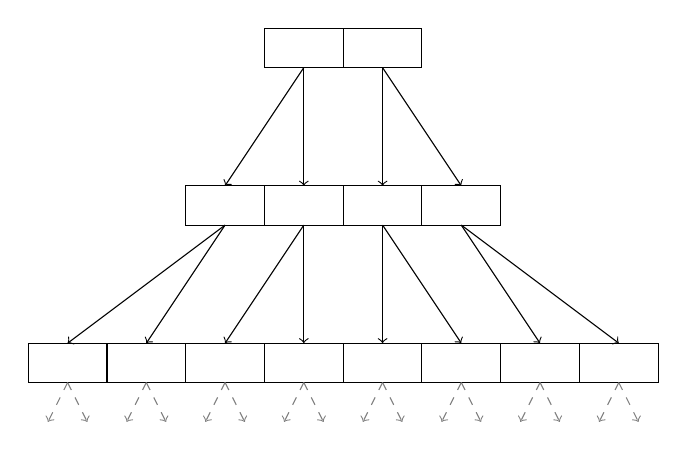
\begin{tikzpicture}
      \foreach \x in {-1, 0} {
        \draw (\x, 0) rectangle (\x+1, 0.5);
      }

      \foreach \x in {-2, -1, 0, 1} {
        \draw (\x, -2) rectangle (\x+1, -1.5);
      }

      \foreach \x in {-4, -3, -2, -1, 0, 1, 2, 3} {
        \draw (\x, -4) rectangle (\x+1, -3.5);
        \draw[->, dashed, gray] (\x+0.5, -4) -- (\x+0.75, -4.5);
        \draw[->, dashed, gray] (\x+0.5, -4) -- (\x+0.25, -4.5);
      }

      \draw[->] (-0.5, 0) to (-1.5,-1.5);
      \draw[->] (-0.5, 0) to (-0.5,-1.5);
      \draw[->] (+0.5, 0) to (+1.5,-1.5);
      \draw[->] (+0.5, 0) to (+0.5,-1.5);

      \draw[->] (-0.5, -2) to (-1.5,-3.5);
      \draw[->] (-0.5, -2) to (-0.5,-3.5);
      \draw[->] (+0.5, -2) to (+1.5,-3.5);
      \draw[->] (+0.5, -2) to (+0.5,-3.5);
      \draw[->] (-1.5, -2) to (-2.5,-3.5);
      \draw[->] (-1.5, -2) to (-3.5,-3.5);
      \draw[->] (+1.5, -2) to (+2.5,-3.5);
      \draw[->] (+1.5, -2) to (+3.5,-3.5);
    \end{tikzpicture}
  \end{figure}


  \begin{lem}
    The constructed function is a PRF.
  \end{lem}
  \begin{prv}
    Define the following games.
    \begin{itemize}
      \item $\mathrm{Hybrid}_0$ is the "Real" experience PRF game.
      \item $\mathrm{Hybrid}_j$ is defined with the following changes:
        \begin{itemize}
          \item at the outset of the game, the challenger initializes an empty table $T$,
          \item given a query $x_1 \ldots x_m$, the challenger executes the following algorithm:
            \begin{itemize}
              \item it looks at whether $(x_1 \ldots x_j , \mathsf{tmp}_{x_1 -\!\!- x_j}) \in T$, if so, define $\mathsf{tmp} := \mathsf{tmp}_{x_1 -\!\!-x_j}$, otherwise it samples $\mathsf{tmp} \gets \mathcal{U}(\{0,1\}^{2n})$ and appends $(x_1\ldots x_j, \mathsf{tmp})$ to $T$.
                (this is ta lazy sampling of a uniform function $\{0,1\}^j \to \{0,1\}^{2n}$).
              \item For $i = j + 1\ldots m$, it updates $\mathsf{tmp} \gets G(\mathsf{tmp}_{1 -\!\!- n})$ if $x_{j+1} $ is $0$, and the result of $G$ on the other half if $x_{j+1} = 1$.
            \end{itemize}
        \end{itemize}
        This way, the game $\mathrm{Hybrid}_j$ is the initial game except that we "cut off" the first $j$ levels of the tree of calls to $G$, and replace them with uniform random values.
    \end{itemize}
    For $j = m$, the game $\mathrm{Hybrid}_m$ is exactly the "Ideal" experience of the PRF game.
    We can bound the advantage using the triangular inequality:
    \begin{align*}
    \mathrm{Adv}_\mathrm{PRF}(\mathcal{A})
    &= \big| \Pr[\mathcal{A} \xrightarrow{\text{Real}} 1] - \Pr[\mathcal{A} \xrightarrow{\text{Ideal}} 1] \big| \\
    &\le \sum_{j=1}^m \big| \Pr[\mathcal{A} \xrightarrow{\mathrm{Hybrid}_j} 1] - \Pr[\mathcal{A} \xrightarrow{\mathrm{Hybrid}_{j+1}} 1] \big|
    .\end{align*}
    We have $m$ hybrids.


    Continuing with hybrid games, we define
    \begin{itemize}
      \item $\mathrm{Hybrid}_{j,\ell}$ to be the same game as $\mathrm{Hybrid}_j$ except that, for the first $\ell$ prefixes $x_i \ldots x_{j+1}$ that are queried, use $\mathrm{Hybrid}_{j+1}$, for the next ones, use $\mathrm{Hybrid}_j$.
        Here, $\ell \in \llbracket 0, q_{j+1}\rrbracket$ where $q_{j+1}$ is the number of $(n-j-1)$-prefixes that occur in the queries from the adversary.
    \end{itemize}
    The number of $\mathrm{Hybrid}_{j,\ell}$'s games is no larger than the number of queries made by $\mathcal{A}$, and $q$ is smaller than the run-time of $\mathcal{A}$, it is polynomial.
    We also have that
    \[
    \mathrm{Adv}_{\mathrm{PRF}}(\mathcal{A}) \le \sum_{j=1}^m \sum_{\ell=1}^{q_{j+1}} \big|
    \Pr[\mathcal{A} \xrightarrow{\mathrm{Hybrid}_{j,\ell}} 1]
    -
    \Pr[\mathcal{A} \xrightarrow{\mathrm{Hybrid}_{j,\ell-1}} 1]
    \big|
    .\]
    The difference between $\mathrm{Hybrid}_{j, \ell}$ and $\mathrm{Hybrid}_{j, \ell+1}$ is exactly one call to $G$ on a uniform input.
    Assuming $G$ is a secure  PRG, this advantage is $\mathrm{negl}(n) = n^{-\omega(1)}$.
    Thus:
    \[
      \mathrm{Adv}_\mathrm{PRF}(\mathcal{A}) \le n^{-\omega(1)} \times m \times \max(q_{j+1}) \le n^{-\omega(1)} \times \underbrace{m \times q}_{\mathrm{poly}(n)} \le n^{-\omega(1)}
    .\]
    (The number of hybrid games must be less than a polynomial in $n$.)
  \end{prv}

  As a consequence, we have the following implications:
  \[
  \begin{tikzcd}
    \text{DDH} \arrow[Rightarrow]{dr}{} \\
    & \text{PRG} \arrow[Rightarrow, bend left]{r}{} & \text{PRF} \arrow[Rightarrow, bend left]{l}{}\\
    \text{LWE} \arrow[Rightarrow]{ur}{} \\
  \end{tikzcd}
  .\]
  These PRFs are not used in practice: for basic PRFs, we use ad-hoc constructions, for PRFs with more advanced functionalities, we direction constructions from LWE and DDH can be interesting.


  \section{Key homomorphic PRF.}

  Can we construct a PRF such that with the following property?
  \[
  F(k_1 \oplus k_2, x) = F(k_1, x) \oplus F(k_2, x)
  .\]

  We can make an ad-hoc construction, the old default PRF is DES (deterministic encryption standard).
  DES  is based on a Feistel network with \textbf{16 rounds} (with distinct keys for every round, all derived from the "master" key).


  \begin{figure}
    \centering
    \begin{tikzpicture}
      \node (l0) at (-2, 0) {$\mathsf{left}_0$};
      \node (r0) at (2, 0) {$\mathsf{right}_0$};
      \draw (-0.5, -0.25) rectangle (-3.5, 0.25);
      \draw (0.5, -0.25) rectangle (3.5, 0.25);

      \draw (2, -0.25) -- (2, -3) -- (-2, -3) -- (-2, -3.75);

      \node (l0) at (-2, -4) {$\mathsf{left}_0$};
      \node (r0) at (2, -4) {$\mathsf{right}_0$};
      \draw (-0.5, -3.75) rectangle (-3.5, -4.25);
      \draw (0.5, -3.75) rectangle (3.5, -4.25);
    \end{tikzpicture}
  \end{figure}

  A \textit{Feistel network} gives a permutation even if $f_k$ is not a permutation.

  In the one presented above, we have $\mathsf{right}_0 = \mathsf{left}_1$, and $\mathsf{left}_0 = f_k(\mathsf{left}_1) \oplus \mathsf{right}_1$.

  A PRP is a pseudo random permutation that come in two kinds: weak and strong.
  \begin{itemize}
    \item A \textit{weak PRP} is defined like a PRF except that $F(k, -)$ is a permutation for any key $k$.
    \item A \textit{strong PRP} is a weak PRP except that $F(k, -)^{-1}$ should be efficient and the adversary is  given query access to both $F(k, -)$ and  $F(k, -)^{-1}$.
  \end{itemize}

  We can consider five exercises:
  \begin{itemize}
    \item a PRF and a two-round Feistel network doesn't define a weak PRP ;
    \item a PRF and a three-round Feistel network does define a weak PRP ;
    \item a PRF and a four-round Feistel network doesn't define a strong PRP ;
    \item a PRF and a five-round Feistel network does define a strong PRP.
  \end{itemize}

  In practice today, people use AES which is not based on a Feistel network (the key size in AES is $128$, $192$ or $256$).

  How do we encrypt with a PRF $F : \{0,1\}^n \times \{0,1\}^n \to \{0,1\}^n$?

  Given $k$ and $m = m_1 m_2 m_3$, we could encrypt it as 
  \[
  F(k, m_1) || F(k, m_2) || F(k, m_3)
  .\]
  DON'T DO THIS!!
  The adversary can see of two $m_i$'s are the same.
  To avoid this kind of attacks, it is necessary that the encryption is randomized.


  An encryption scheme $(\mathrm{Enc}, \mathrm{Dec})$ is \textit{IND-CPA} (\textit{undistinguishable under chosen plain-text attacks}) secure for multiple messages of the advantage of any polynomial-time adversary $\mathcal{A}$ is negligible where the game is the following.
  \begin{itemize}
    \item The challenger gets a random uniform bit $b \in \{0,1\}$.
    \item The challenger chooses a key $k \in \{0,1\}^n$ uniformly.
    \item The adversary sends two messages $(m^{0}_0, m^{0}_1)$ to $\mathcal{C}$.
    \item The challenger encodes $m^0_b$ using $k$ and sends it to $\mathcal{A}$.
    \item The adversary can send as many two-messages packets $(m_0^i, m_1^i)$ as it wants, and the challenger will give the cipher-text corresponding to $m^{i}_b$.
    \item Finally, the adversary will return a guess $b'$ for $b$.
  \end{itemize}

  The advantage is defined as:
  \[
    \mathrm{Adv}(\mathcal{A}) := \big| \Pr[\mathcal{A} \to 1  \mid b = 1] - \Pr[\mathcal{A} \to 1  \mid b = 0] \big|
  .\]


  How do we formalize the previous attack?
  Consider three messages $(m_0, m_1, m_2)$.
  Then the attacker will send $(m_0, m_1)$ and $(m_0, m_2)$.
  If the PRF $F$ is deterministic, then $c_0 = c_1$ in the case  $b = 0$.
  This gives a distinguisher.


  The right way to encrypt with a PRF is the following.
  \begin{description}
    \item[Encryption.]
      Given the inputs $(k,m)$, take  $r \gets \mathcal{U}(\{0,1\}^n)$ and output $c = r || m \oplus F(k, r) \in \{0,1\}^{2n}$.
    \item[Decryption.]
      Given $(k, c_1 || c_2)$, output $F(k, c_1) \oplus c_2$.
  \end{description}

  We immediately have that $\mathrm{Dec}(k, \mathrm{Enc}(k, m)) = m$ for any $(k, m)$.

  The intuition for the security proof is the following.
  As the number of queries is less than a polynomial in $n$, it's very unlikely that two queries are being replied to with the same $r$.
  If the $r$s are distinct, then $F(k, r)$ plays the role of a mask and hides $m$.

  If I encrypt a message of length $\ell$ plain-text by using this $t$ times, then the output has size $2 \ell$.

  \textbf{[Something to fill here\ldots]}
\end{document}
